\chapter{Application web}

	\section{Organisation des packages}

		\subsection{Packages}

			%TODO Léa : Image et décrire le but des packages (src)

		\subsection{Resources}

			%TODO Léa : Comme avec les packages mais sur les ressources

	\section{Configuration de l'application}

		\subsection{application.properties}

			L'application web possède un fichier application.properties qui permet de configurer certaines parties de l'application.

			\begin{figure}[H]
				\centering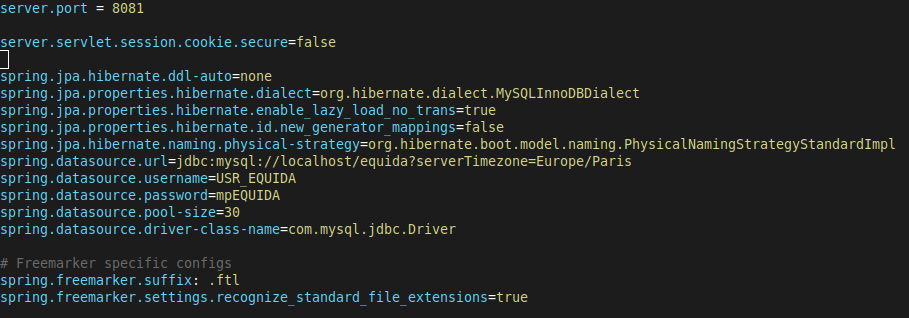
\includegraphics[width=0.85\textwidth, keepaspectratio]{res/application-properties.png}
				\caption{Configuration par application.properties}
			\end{figure}

			Dans ce fichier configure les informations relatives à l'application dans sa globalité, comme le port à utiliser, la configuration pour connexion avec la \bdd{} (nom utilisateur, mot de passe, ip, ...) ou encore la configuration du moteur de template, freemarker en l'occurence.

		\subsection{Configuration par le code}
			\label{subsec:webapp_configCode}

			La configuration de Spring Security est directement faite dans le code source grace à l'utilisation de l'annotation "Configuration".

			\begin{figure}[H]
				\centering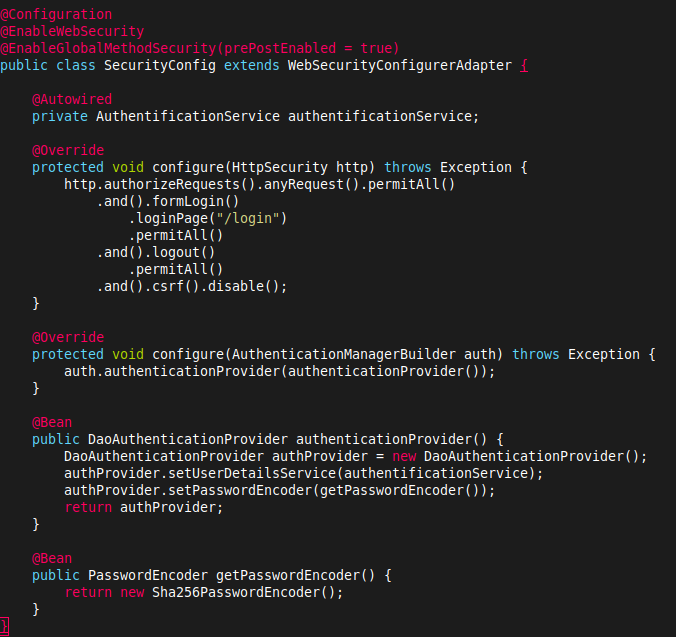
\includegraphics[width=0.75\textwidth, keepaspectratio]{res/SecurityConfig.png}
				\caption{Configuration de Spring Security}
			\end{figure}

			La méthode "void configure(HttpSecurity http)" permet de configurer l'accès aux différentes pages et de changer la configuration des requêtes HTTP. Ainsi, on autorise la connexion sur toutes les pages web, d'autant plus sur login et logout. De cette manière le jour où l'on décidera de changer cette configuration, le code pour autoriser l'accès à "/logout" et "/login" sera déjà présent et empêchera un potentiel oubli.


			\label{par:authentification}
			Les méthodes suivantes sont relatives à l'authentification. La méthode "void configure( AuthenticationManagerBuilder)" permet de changer la méthode d'authentification utilisée par Spring Security. Elle fait appel à "DaoAuthenticationProvider authenticationProvider()" qui retourne le Dao à utiliser. On doit donc fournir le "UserDetailsService" fournis par le module core, c'est à dire "AuthentificationService" (cf : \nameref{sec:core_authentification}), et le "PasswordEncoder" approprié. De ce fait on utilise donc une nouvelle instance de "Sha256PasswordEncoder" (cf : \nameref{subsec:Sha256PasswordEncoder}).

	\section{Fichiers resources}

		\subsection{Freemarker}

			Comme mentionné auparavant, tout les fichiers de freemarker sont contenus dans le dossier "templates" dans les ressources. Il est donc possible d'utiliser les directives propres à ce moteur de template.

			\subsubsection{Page de base}

				%TODO Léa : Expliquer le fonctionnement de la page de base et les macros

			\subsubsection{Page d'erreur}

				%TODO Léa : Expliquer que les pages sont chargés automatiquement par spring et reprenne design de base

			\subsubsection{Fichiers à inclure}

				Le dossier "view/include/" contient des vues communes aux différentes pages. On peut les inclures en utilisant les directives "<\#include ''/>". On retrouve par exemple le fichier lotLister qui permet d'afficher les cartes pour les différents lots.

				\begin{figure}[H]
					\centering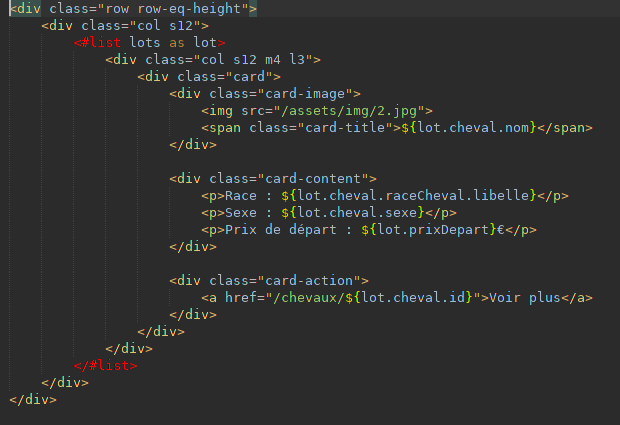
\includegraphics[width=0.75\textwidth, keepaspectratio]{res/include-lotLister.png}
					\caption{Configuration de Spring Security}
				\end{figure}

				Le code reste celui de n'importe quelle autre vue et ne comporte aucune spécificité telle que des directives "<\#macro>".

			\subsubsection{Exemple de page web}

				Ainsi, avec toutes les éléments cités précédemments, on peut créer des vues telles que celle ci :

				\begin{figure}[H]
					\centering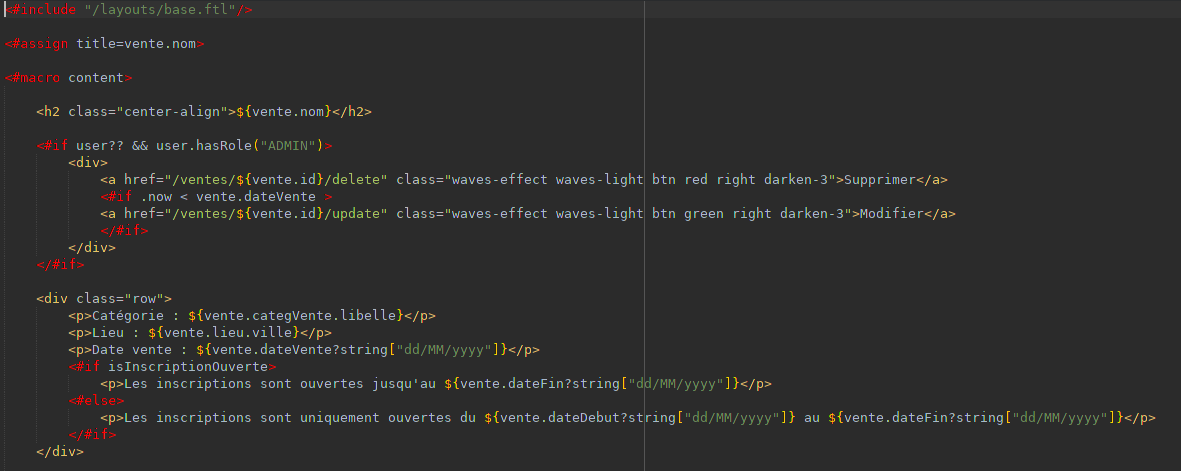
\includegraphics[width=0.85\textwidth, keepaspectratio]{res/view-venteConsulter.png}
					\caption{Code de la vue pour la consultation d'une vente}
				\end{figure}

				On retrouve tout les éléments précédemments cités. L'include de "/layouts/base.ftl" pour reprendre le template de base, un changement de valeur concernant le titre, l'utlisation de la macro "content", ...

		\subsection{Assets (images, js, ...)}

			%TODO Léa : Je sais pas trop... Décrire le fonctionnement général avec un exemple. Si tu as de meilleures idées vas y :)

	\section{Gestion de l'authentification}

		\subsection{Gestion template et controller}

			Un controleur existe afin de gérer l'affichage d'un template freemarker concernant la page de connexion à l'application. Ce controleur se charge uniquement de l'affichage de l'information. En effet, le traitement des identifiants est fait par Spring Security (comme mentionné dans \nameref{subsec:webapp_configCode}).

		\subsection{Interceptor}

			Afin de faciliter la gestion de l'utilisateur actuellement connecté dans le vue ou les controleurs une classe "UserInterceptor" permet de founir automatiquement l'instance de "AuthentificatedUser" à la vue ou au controleur.

			\begin{figure}[H]
				\centering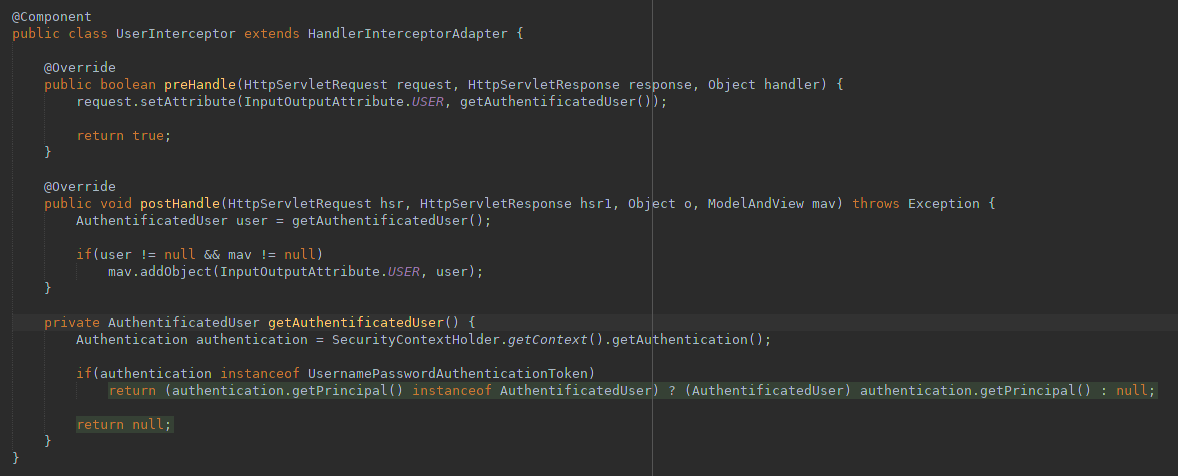
\includegraphics[width=0.85\textwidth, keepaspectratio]{res/UserInterceptor.png}
				\caption{Code de UserInterceptor}
			\end{figure}

			On peut alors avoir accès à la variable "user" dans la vue comme n'importe quelle autre variable fournis par le controleur ou alors dans le controleur en utilisant le paramètre suivant dans une méthode d'un controleurs "@RequestAttribute(name = InputOutputAttribute.USER, required = false) AuthentificatedUser user".

	\section{Exemple Route}

		%TODO Léa : Expliquer les méthodes de l'interface IRoute et donner un exemple de route.

	\section{Exemple Form}

		%TODO Léa : Expliquer la classe mère IForm et donner un exemple de formulaire (Avec Add et Update et le Neutre)

	\section{Classe InputOutputAttribute}

		Cette classe permet la définition de constantes qui seront utilisés au travers de l'application.

		\begin{figure}[H]
			\centering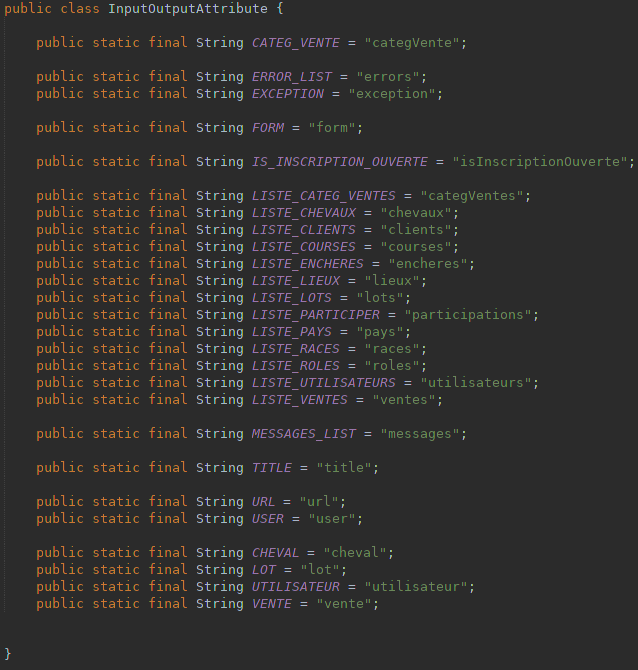
\includegraphics[width=0.65\textwidth, keepaspectratio]{res/InputOutputAttribute.png}
			\caption{Code de InputOutputAttribute}
		\end{figure}

		Elles permettent de garder une unité dans la définition des noms et d'éviter d'éventuelles erreurs d'écriture. Ainsi, lorsque l'on doit fournir une clé de type String on pourra utiliser une des constantes de la classe. Ces constantes sont donc énormément utilisés pour transmettre les informations du controleur vers la vue.

		\begin{figure}[H]
			\centering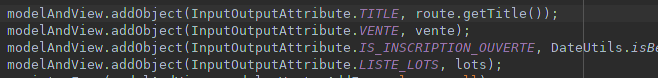
\includegraphics[width=0.75\textwidth, keepaspectratio]{res/InputOutputAttribute-controller.png}
			\caption{Exemple d'utilisation de InputOutputAttribute}
		\end{figure}

	\section{Les Controleurs}

		\subsection{AbstractWebController}

			Cette classe est la classe mère de tout les controleurs. On y définis certaines méthodes comme la possibilité d'ajouter des messages d'erreurs, ou à titres informatifs, qui seront transférés à la vue.

			\begin{figure}[H]
				\centering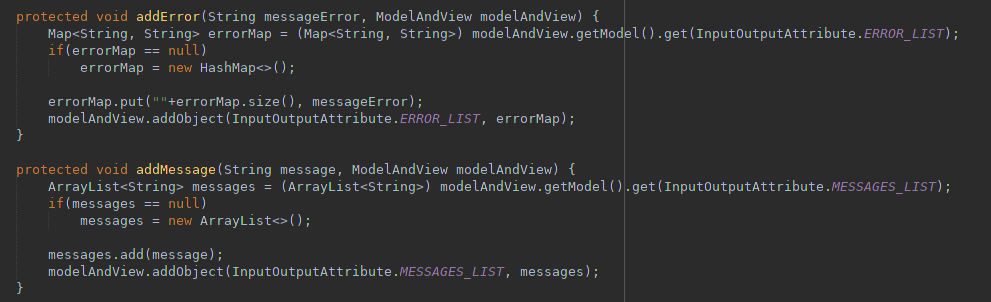
\includegraphics[width=0.85\textwidth, keepaspectratio]{res/AbstractWebController-messages.png}
				\caption{Méthodes pour la gestion des messages}
			\end{figure}

			On y définit aussi la gestion des exception dans lequels on passe les variables necessaires au bon affichage de la vue.

			\begin{figure}[H]
				\centering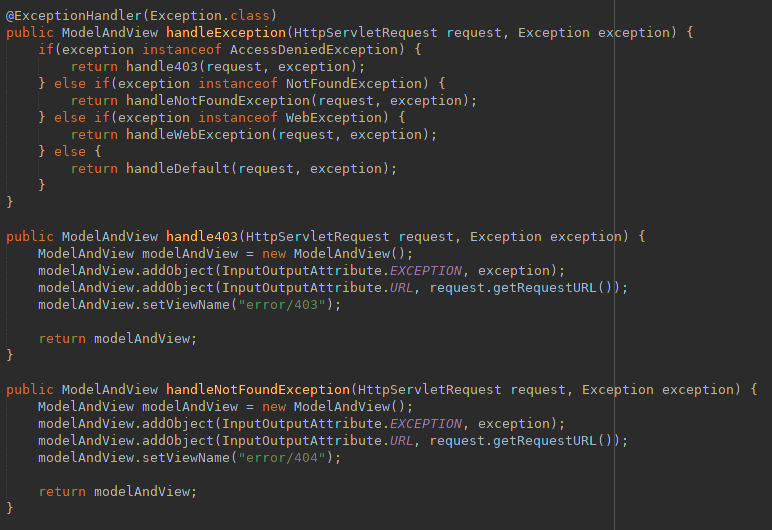
\includegraphics[width=0.75\textwidth, keepaspectratio]{res/AbstractWebController-exception.png}
				\caption{Méthodes pour la gestion des exceptions}
			\end{figure}

			Elle définit aussi 2 méthodes qui permettent de simplifier le code de gestion des formulaires, l'une afin de les créer et de les compléter si besoin, l'autre afin de faciliter la gestion des erreurs sur ceux ci.

			\begin{figure}[H]
				\centering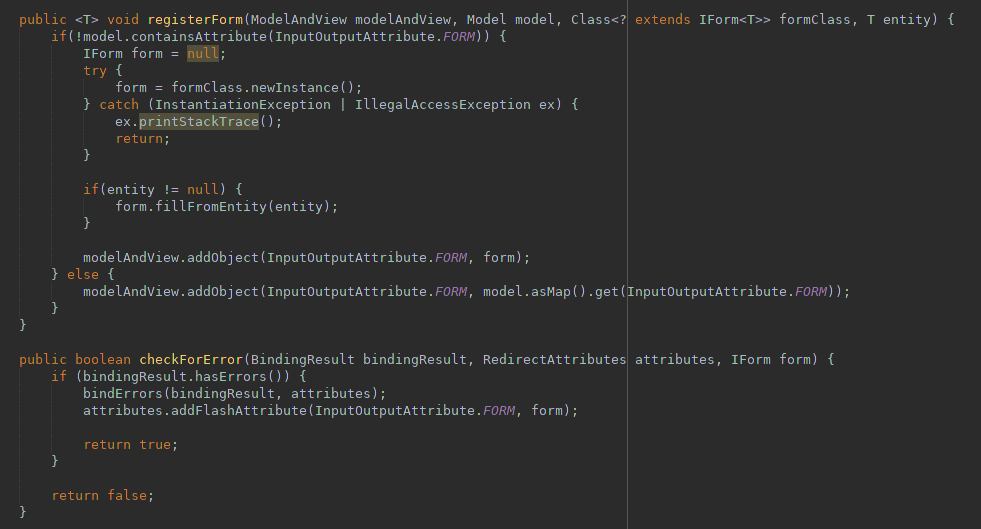
\includegraphics[width=0.80\textwidth, keepaspectratio]{res/AbstractWebController-form.png}
				\caption{Méthodes pour la gestion des form}
			\end{figure}

		\subsection{Exemple Controller}

			%TODO Léa : Donner un exemple de controller
